\begin{center}
\Huge
Differentialligninger og grafer
\end{center}


\section*{Grafer}
\stepcounter{section}

Vi arbejdede sidst med tre typer af differentialligninger.
\begin{align*}
	y' &= k,\\
	y' &= ky,  \textnormal{ og}\\
	y' &= b-ay.
\end{align*}

Vi kan se disse tre differentialligninger tegnet med $y$ langs førsteaksen og $y'$ langs andenaksen på Fig. \ref{fig:diffs}
\begin{figure}[H]
	\centering
	\resizebox{0.45\textwidth}{!}
	{
	\begin{tikzpicture}
		\begin{axis}
			[axis lines = middle, 
			xmin = -1, xmax = 5,
			ymin = -1, ymax = 5,
			ticks = none, 
			xlabel = {$y$}, ylabel = {$y'$}
			]
			\addplot[thick, color = blue!40] {3};			
		\end{axis}
	\end{tikzpicture}
	}
	\resizebox{0.45\textwidth}{!}
	{
	\begin{tikzpicture}
		\begin{axis}
			[axis lines = middle, 
			xmin = -1, xmax = 5,
			ymin = -1, ymax = 5,
			ticks = none, 
			xlabel = {$y$}, ylabel = {$y'$}
			]
			\addplot[thick, color = blue!40] {x};			
		\end{axis}
	\end{tikzpicture}
	}
	\resizebox{0.45\textwidth}{!}
	{
	\begin{tikzpicture}
		\begin{axis}
			[axis lines = middle, 
			xmin = -1, xmax = 5,
			ymin = -1, ymax = 5,
			ticks = none, 
			xlabel = {$y$}, ylabel = {$y'$}
			]
			\addplot[thick, color = blue!40, domain = 0:4] {4-x};			
		\end{axis}
	\end{tikzpicture}
	}
	\caption{Differentialligningerne $y'=k$, $y' = ky$ og $y' = b-ay$ henholdsvist.}
	\label{fig:diffs}
\end{figure}

\begin{exa}
	Vi har repræsenteret en differentialligning grafisk ved
	\begin{center}
		\begin{tikzpicture}
		\begin{axis}
			[axis lines = middle, 
			xmin = -1, xmax = 5,
			ymin = -1, ymax = 5,
			xlabel = {$y$}, ylabel = {$y'$}
			]
			\addplot[thick, color = blue!40] {3};			
		\end{axis}
		\end{tikzpicture}
	\end{center}
	Denne differentialligning er derfor givet ved
	\begin{align*}
		y' = 3, 
	\end{align*}
	og derfor er den fuldstændige løsning givet ved
	\begin{align*}
		y(x) = 3x+c.
	\end{align*}
\end{exa}
\begin{exa}
	En differentialligning er repræsenteret grafisk ved
	\begin{center}
		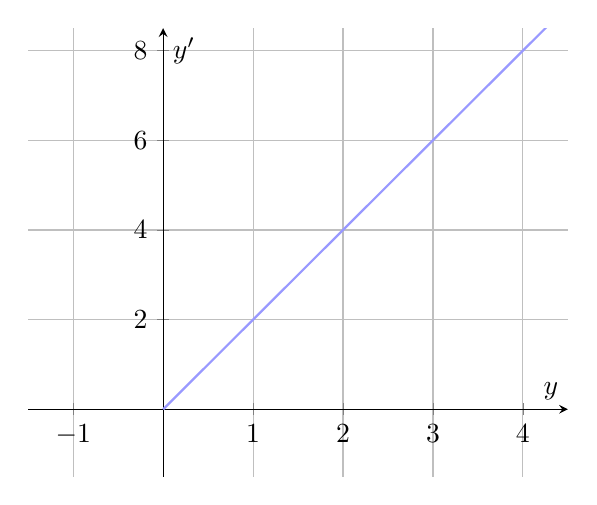
\begin{tikzpicture}
		\begin{axis}
			[axis lines = middle, 
			xmin = -1.5, xmax = 4.5,
			ymin = -1.5, ymax = 8.5,
			xlabel = {$y$}, ylabel = {$y'$},
			grid
			]
			\addplot[thick, color = blue!40, domain = 0:4.5] {2*x};			
		\end{axis}
		\end{tikzpicture}
	\end{center}
	Af grafen kan vi se, at differentialligningen lyder
	\begin{align*}
		y' = 2y,
	\end{align*}
	og derfor har differentialligningen den fuldstændige løsning
	\begin{align*}
		y(x) = ce^{2x}.
	\end{align*}
\end{exa}


\begin{exa}
	Vi har følgende grafiske repræsentation for en differentialligning.
	\begin{center}
		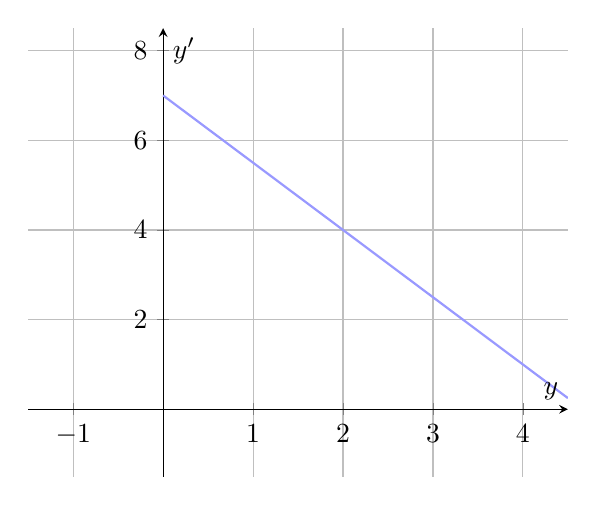
\begin{tikzpicture}
		\begin{axis}
			[axis lines = middle, 
			xmin = -1.5, xmax = 4.5,
			ymin = -1.5, ymax = 8.5,
			xlabel = {$y$}, ylabel = {$y'$},
			grid
			]
			\addplot[thick, color = blue!40, domain = 0:4.5] {7-1.5*x};			
		\end{axis}
		\end{tikzpicture}
	\end{center}
	Af grafen kan vi se, at differentialligningen lyder
	\begin{align*}
		y' = 7-\frac{3}{2}y,
	\end{align*}
	og derfor har differentialligningen den fuldstændige løsning
	\begin{align*}
		y(x) = \frac{14}{3} + ce^{-\frac{3}{2}x}.
	\end{align*}
\end{exa}

\section*{Opgave 1}
Bestem fuldstændige løsninger til følgende grafisk repræsenterede differentialligninger
\begin{center}
	\resizebox{0.45\textwidth}{!}
	{
		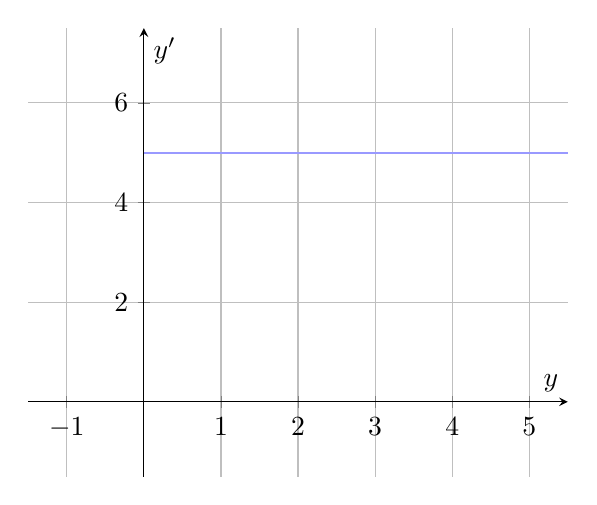
\begin{tikzpicture}
		\begin{axis}
			[axis lines = middle, 
			xmin = -1.5, xmax = 5.5,
			ymin = -1.5, ymax = 7.5,
			xlabel = {$y$}, ylabel = {$y'$},
			grid
			]
			\addplot[thick, color = blue!40, domain = 0:5.5] {5};			
		\end{axis}
		\end{tikzpicture}
	}
	\resizebox{0.45\textwidth}{!}
	{
		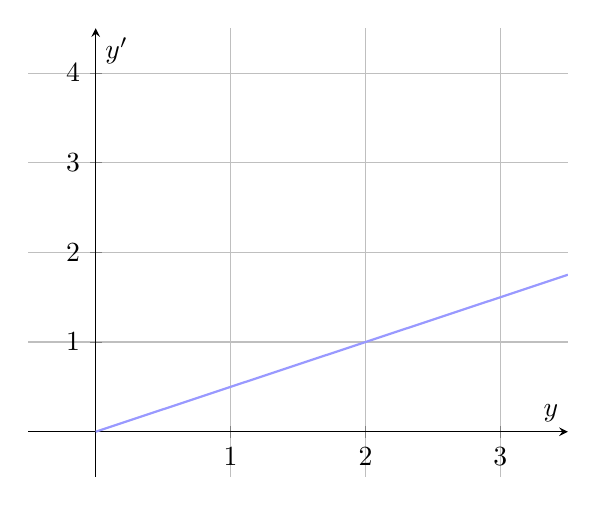
\begin{tikzpicture}
		\begin{axis}
			[axis lines = middle, 
			xmin = -0.5, xmax = 3.5,
			ymin = -0.5, ymax = 4.5,
			xlabel = {$y$}, ylabel = {$y'$},
			grid
			]
			\addplot[thick, color = blue!40, domain = 0:3.5] {0.5*x};			
		\end{axis}
		\end{tikzpicture}
	}
	\resizebox{0.45\textwidth}{!}
	{
		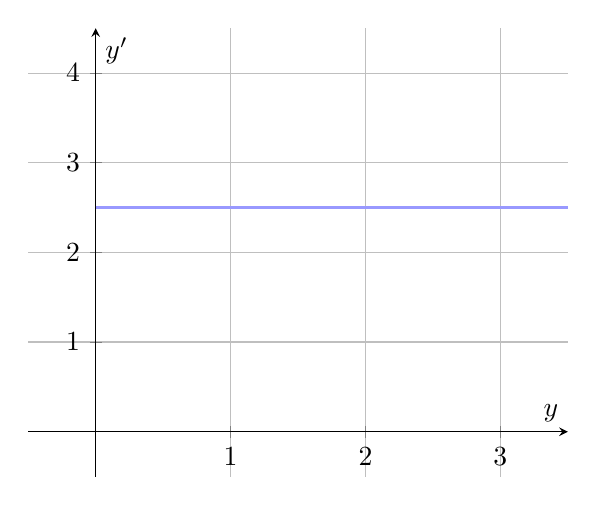
\begin{tikzpicture}
		\begin{axis}
			[axis lines = middle, 
			xmin = -0.5, xmax = 3.5,
			ymin = -0.5, ymax = 4.5,
			xlabel = {$y$}, ylabel = {$y'$},
			grid
			]
			\addplot[thick, color = blue!40, domain = 0:3.5] {2.5};			
		\end{axis}
		\end{tikzpicture}
	}
	\resizebox{0.45\textwidth}{!}
	{
		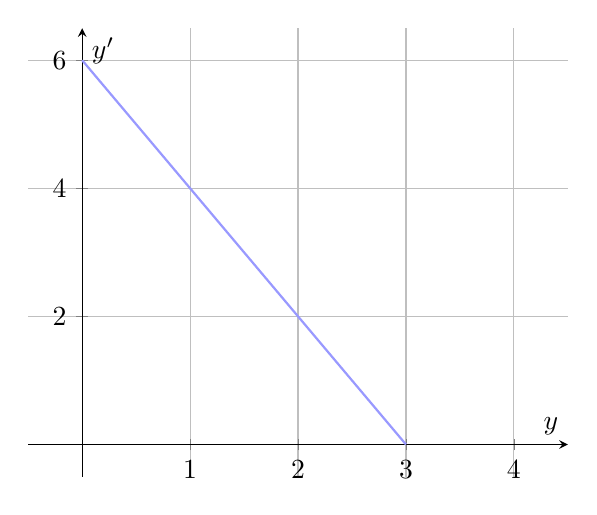
\begin{tikzpicture}
		\begin{axis}
			[axis lines = middle, 
			xmin = -0.5, xmax = 4.5,
			ymin = -0.5, ymax = 6.5,
			xlabel = {$y$}, ylabel = {$y'$},
			grid
			]
			\addplot[thick, color = blue!40, domain = 0:3] {6-2*x};			
		\end{axis}
		\end{tikzpicture}
	}
	\resizebox{0.45\textwidth}{!}
	{
		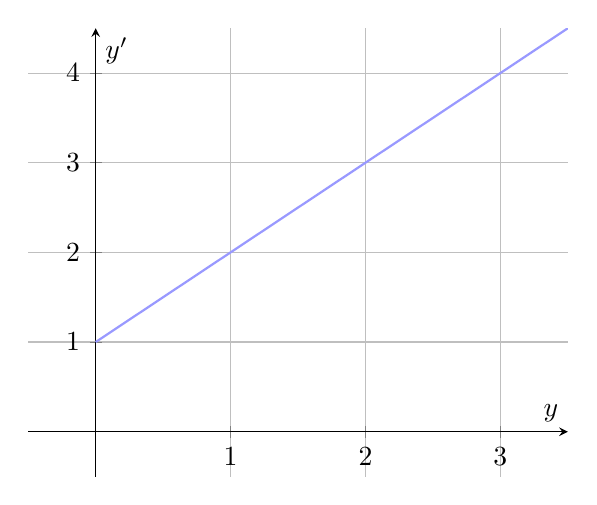
\begin{tikzpicture}
		\begin{axis}
			[axis lines = middle, 
			xmin = -0.5, xmax = 3.5,
			ymin = -0.5, ymax = 4.5,
			xlabel = {$y$}, ylabel = {$y'$},
			grid
			]
			\addplot[thick, color = blue!40, domain = 0:3.5] {1+x};			
		\end{axis}
		\end{tikzpicture}
	}
	\resizebox{0.45\textwidth}{!}
	{
		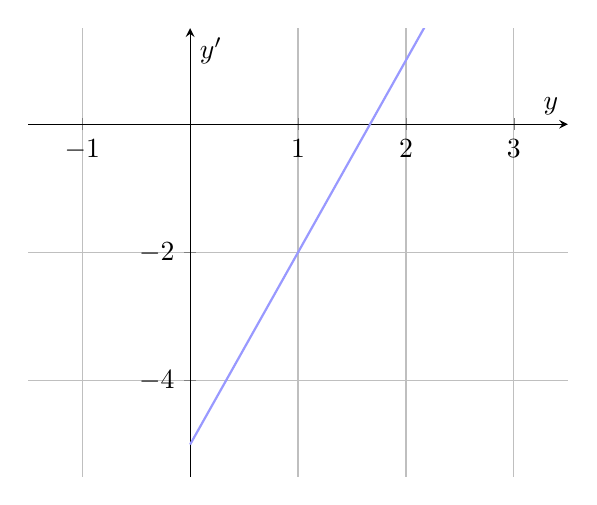
\begin{tikzpicture}
		\begin{axis}
			[axis lines = middle, 
			xmin = -1.5, xmax = 3.5,
			ymin = -5.5, ymax = 1.5,
			xlabel = {$y$}, ylabel = {$y'$},
			grid
			]
			\addplot[thick, color = blue!40, domain = 0:3.5] {-5+3*x};			
		\end{axis}
		\end{tikzpicture}
	}
	
\end{center}

\section*{Opgave 2}
\begin{enumerate}[label=\roman*)]
	\item Bestem den partikulære løsning til differentialligningen repræsenteret på følgende graf, der opfylder, at den 		    går gennem punktet $(0,7)$.
	\begin{center}
		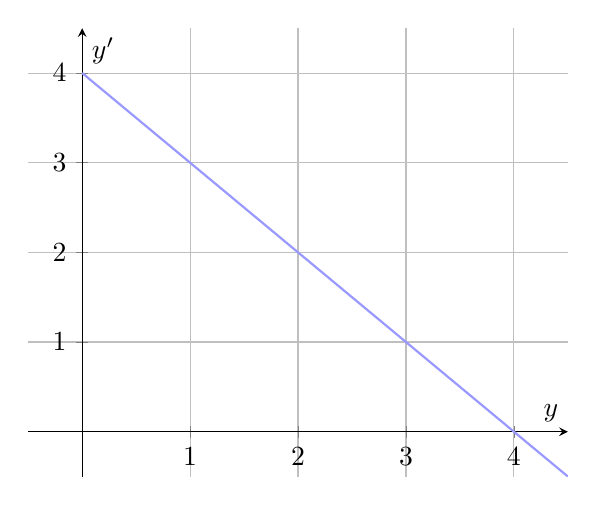
\begin{tikzpicture}
		\begin{axis}
			[axis lines = middle, 
			xmin = -0.5, xmax = 4.5,
			ymin = -0.5, ymax = 4.5,
			xlabel = {$y$}, ylabel = {$y'$},
			grid
			]
			\addplot[thick, color = blue!40, domain = 0:4.5] {4-x};			
		\end{axis}
		\end{tikzpicture}
	\end{center}
	\item Bestem en partikulær løsning til differentialligningen repræsenteret på følgende graf, der går gennem punktet 
	$(0,\sqrt{2})$.
	\begin{center}
		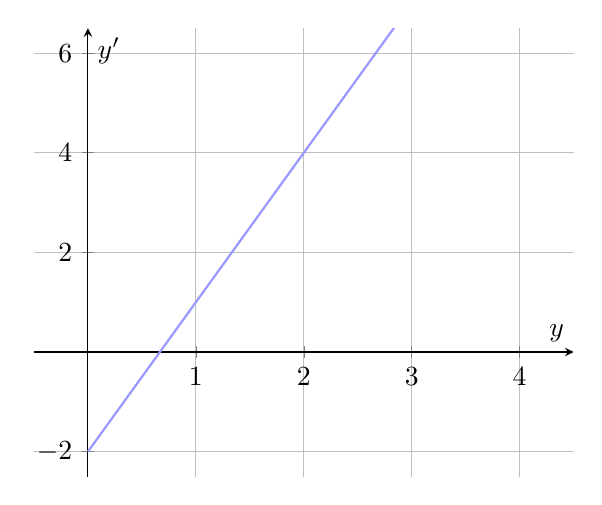
\begin{tikzpicture}
		\begin{axis}
			[axis lines = middle, 
			xmin = -0.5, xmax = 4.5,
			ymin = -2.5, ymax = 6.5,
			xlabel = {$y$}, ylabel = {$y'$},
			grid
			]
			\addplot[thick, color = blue!40, domain = 0:4.5] {-2+3*x};			
		\end{axis}
		\end{tikzpicture}
	\end{center}
\end{enumerate}
\section*{Opgave 3}
\begin{enumerate}[label=\roman*)]
	\item En ret linje $y' = b-ay$ går gennem punkterne $(1,3)$ og $(3,9)$. Bestem den fuldstændige løsning $y$ til den
	differentialligning, der er repræsenteret ved denne rette linje.
	\item En ret linje $y' = b-ay$ går gennem punkterne $(1,2)$ og $(2,4)$. Bestem den partikulære løsning $y$ til den 
	differentialligning, der er repræsenteret ved denne rette linje.
\end{enumerate}

\section*{Opgave 4}
\begin{enumerate}[label=\roman*)]
	\item Følgende sammenhæng mellem $y$ og $y'$ er givet.
	\begin{center}
	\begin{tabular}{c|c|c|c|c|c|c}
		$y$ & 1.3 & 3.2 & 5.7 & 6.9 & 10.68 & 11.97\\
		\hline
		 $y'$ & 69.5 & 58.1 & 42.4 & 44.7 & 18.4 & 28.35
	\end{tabular}
	\end{center}
	Det antages, at sammenhængen mellem $y$ og $y'$ er givet ved
	\begin{align*}
		y' = b-ay.
	\end{align*}
	Brug datasættet til at bestemme den fuldstændige løsning $y$. 
\end{enumerate}

\section*{Opgave 5}
	Et objekt med en temperatur på $100^\circ$C stilles i et lokale med en temperatur på $19^\circ$C. Det er oplagt, at temperaturen falder langsomme og langsommere jo nærmere
	temperaturen kommer på den omkringliggende temperatur. Vi antager, at temperaturfaldets hastighed er proportional med objektets temperatur eller mere præcist, at 
	temperaturen og temperaturfaldet opfylder differentialligningen
	\begin{align*}
		y' = -k(y-19) = -ky+19k.
	\end{align*}
	\begin{enumerate}[label=\roman*)]
		\item Bestem den fuldstændige løsning til differentialligningen. 
		\item Udnyt, at $y(0) = 100$ til at bestemme konstanten $c$. 
		\item Udnyt, at temperaturen efter 5 minutter er $80^\circ$C til at bestemme $k$. 
		\item Opskriv modellen $y(t)$ for temperaturen af objektet. 
	\end{enumerate}